\chapter{大脑指挥}\label{ch:g5:brain-in-command}

一个球朝你飞来，你接住了它。只用了半秒，
完全没有经过思考——但在这半秒之内，你的眼睛报告了
一个飞行中的物体，有什么东西算出了它的路线，还有几十块
\omterm{def:g3:bones-and-muscles:muscle}{肌肉}接到指令，恰好完成了这一次接球。
这个“东西”就是\omterm{def:g5:brain-in-command:system}{大脑}，本章将沿着身体的
\omterm{def:g5:brain-in-command:system}{神经}线路，追踪它发出的指令。

\section{指令网络}

\begin{definition}[神经系统]\label{def:g5:brain-in-command:system}
\emph{神经系统}\index{神经系统}是身体的
指令网络：
\begin{itemize}
  \item \emph{大脑}\index{大脑}，位于\omterm{def:g3:bones-and-muscles:skeleton}{颅骨}的保护之中，
        （\cref{def:g3:bones-and-muscles:skeleton}），是
        中枢：接收所有报告，并发出所有指令；
  \item \emph{脊髓}\index{脊髓}，一条粗壮的
        神经组织索，从大脑向下延伸，穿行于
        \omterm{def:g4:classifying-animals:vertebrate}{脊柱}的保护柱之内；
  \item \emph{神经}\index{神经}，白色的细丝，
        从大脑和脊髓\omterm{def:g1:plants-around-us:tree}{分支}延伸到每一个器官，
        负责传递信息——最快的可超过
        \qty{100}{m/s} 以上。
\end{itemize}
\end{definition}

\begin{proposition}[报告、决定、指令]\label{prop:g5:brain-in-command:loop}
每一个动作都遵循同一个循环
（\cref{prop:g1:the-five-senses:brain}中是它的最初草图）：
\begin{enumerate}
  \item \emph{\omterm{def:g1:the-five-senses:sense}{感觉器官}}发出报告：\omterm{def:g5:brain-in-command:system}{神经}把它们的
        信息\emph{传送至}\omterm{def:g5:brain-in-command:system}{大脑}；
  \item \emph{\omterm{def:g5:brain-in-command:system}{大脑}}综合各项报告，作出决定，
        并发出指令；
  \item \omterm{def:g5:brain-in-command:system}{神经}把指令\emph{从}\omterm{def:g5:brain-in-command:system}{大脑}传送到
        \emph{\omterm{def:g3:bones-and-muscles:muscle}{肌肉}}（\cref{def:g3:bones-and-muscles:muscle}），
        \omterm{def:g3:bones-and-muscles:muscle}{肌肉}接到指令后收缩。
\end{enumerate}
\omterm{def:g1:the-five-senses:sense}{感觉器官}负责报告，\omterm{def:g3:bones-and-muscles:muscle}{肌肉}负责执行——两者都不作决定。
\end{proposition}
\admitted

\begin{omfigure}
\begin{tikzpicture}
  % eye
  \draw[thick] (-0.7,1.7) ellipse (0.5 and 0.28);
  \fill[omDef] (-0.58,1.7) circle (0.13);
  \node[font=\small, align=center] (eye) at (-0.7,0.85)
    {眼睛看到 \\ 球};
  % brain
  \draw[thick, omDef, fill=omDef!8, rounded corners=8pt]
    (3.2,1.15) rectangle (6.4,2.45);
  \node[font=\small\bfseries, omDef] at (4.8,2.05) {大脑};
  \node[font=\footnotesize] at (4.8,1.55) {决定接球};
  % muscle
  \draw[thick, omThm, fill=omThm!15]
    (9.6,1.5) .. controls (10.0,1.85) and (10.6,1.85) .. (11.0,1.55)
    .. controls (10.6,1.35) and (10.0,1.35) .. (9.6,1.5);
  \node[font=\small, align=center] at (10.3,0.85)
    {手臂肌肉 \\ 收缩};
  % arrows
  \draw[->, very thick, omMeth] (-0.1,1.7) -- (3.1,1.8)
    node[pos=0.42, above=2pt, font=\footnotesize, omMeth]
    {沿神经报告};
  \draw[->, very thick, omProp] (6.5,1.8) -- (9.5,1.6)
    node[pos=0.5, above=2pt, font=\footnotesize, omProp]
    {沿神经发出指令};
\end{tikzpicture}

{\small 每一个动作的循环：向\omterm{def:g5:brain-in-command:system}{大脑}报告、作出决定、
向\omterm{def:g3:bones-and-muscles:muscle}{肌肉}发出指令。}
\end{omfigure}

\begin{example}[慢放这次接球]\label{ex:g5:brain-in-command:catch}
把这半秒慢慢重放：眼睛持续追踪球并报告，
\omterm{def:g5:brain-in-command:system}{大脑}不断比较一份份报告，算出
球将落在哪里；指令源源发往腿部（向左迈一步）、
躯干（前倾）、手臂和手指（张开——再合拢）。没有任何
一个器官“接住了球”：眼睛、\omterm{def:g5:brain-in-command:system}{大脑}和\omterm{def:g3:bones-and-muscles:muscle}{肌肉}
各自扮演了
\cref{prop:g5:brain-in-command:loop}中的角色。
\end{example}

\begin{remark}[不止于运动]\label{rem:g5:brain-in-command:more}
同一个\omterm{def:g5:brain-in-command:system}{大脑}在接球的同时，也储存你的记忆，
让你的注意力停留在这一页上，夜里做梦——还
负责你从不曾留意的工作：它让\omterm{def:g4:breathing:movements}{呼吸}日夜不停
（见\cref{def:g4:breathing:movements}），并根据身体的需要
调节心跳的节奏
（见\cref{ex:g4:heart-and-blood:effort}）。有些指令由你自己发出，
另一些则由\omterm{def:g5:brain-in-command:system}{大脑}替你发出。
\end{remark}

\section{测量循环：反应时间}

\begin{definition}[反应时间]\label{def:g5:brain-in-command:reaction}
这个循环很快，但并非瞬间完成：报告、决定和指令
各需要一定时间。从信号出现到身体作出反应之间的延迟，
就是\emph{反应时间}\index{反应时间}——对于简单的任务（接住、按下、抓取），
熟练的人约需五分之一秒，
儿童则稍长一些。
\end{definition}

\begin{method}[尺子测试]\label{met:g5:brain-in-command:ruler}
只用一把尺子、不借助其他仪器测量\omterm{def:g5:brain-in-command:reaction}{反应时间}：
\begin{enumerate}
  \item 让同伴竖直拿着一把尺子，零刻度朝下，
        悬在你张开的拇指和食指之间；
  \item 同伴不作预告地松开手，你尽快接住
        尺子；
  \item 读出接住的位置：尺子滑过的厘米数越少，
        你的循环就越快；
  \item 多做几次，记下你的典型数值——
        单次测量的结果波动很大。
\end{enumerate}
下落的尺子把时间换算为厘米：约
$\qty{15}{cm}$ 对应六分之一秒。
\end{method}

\begin{omfigure}
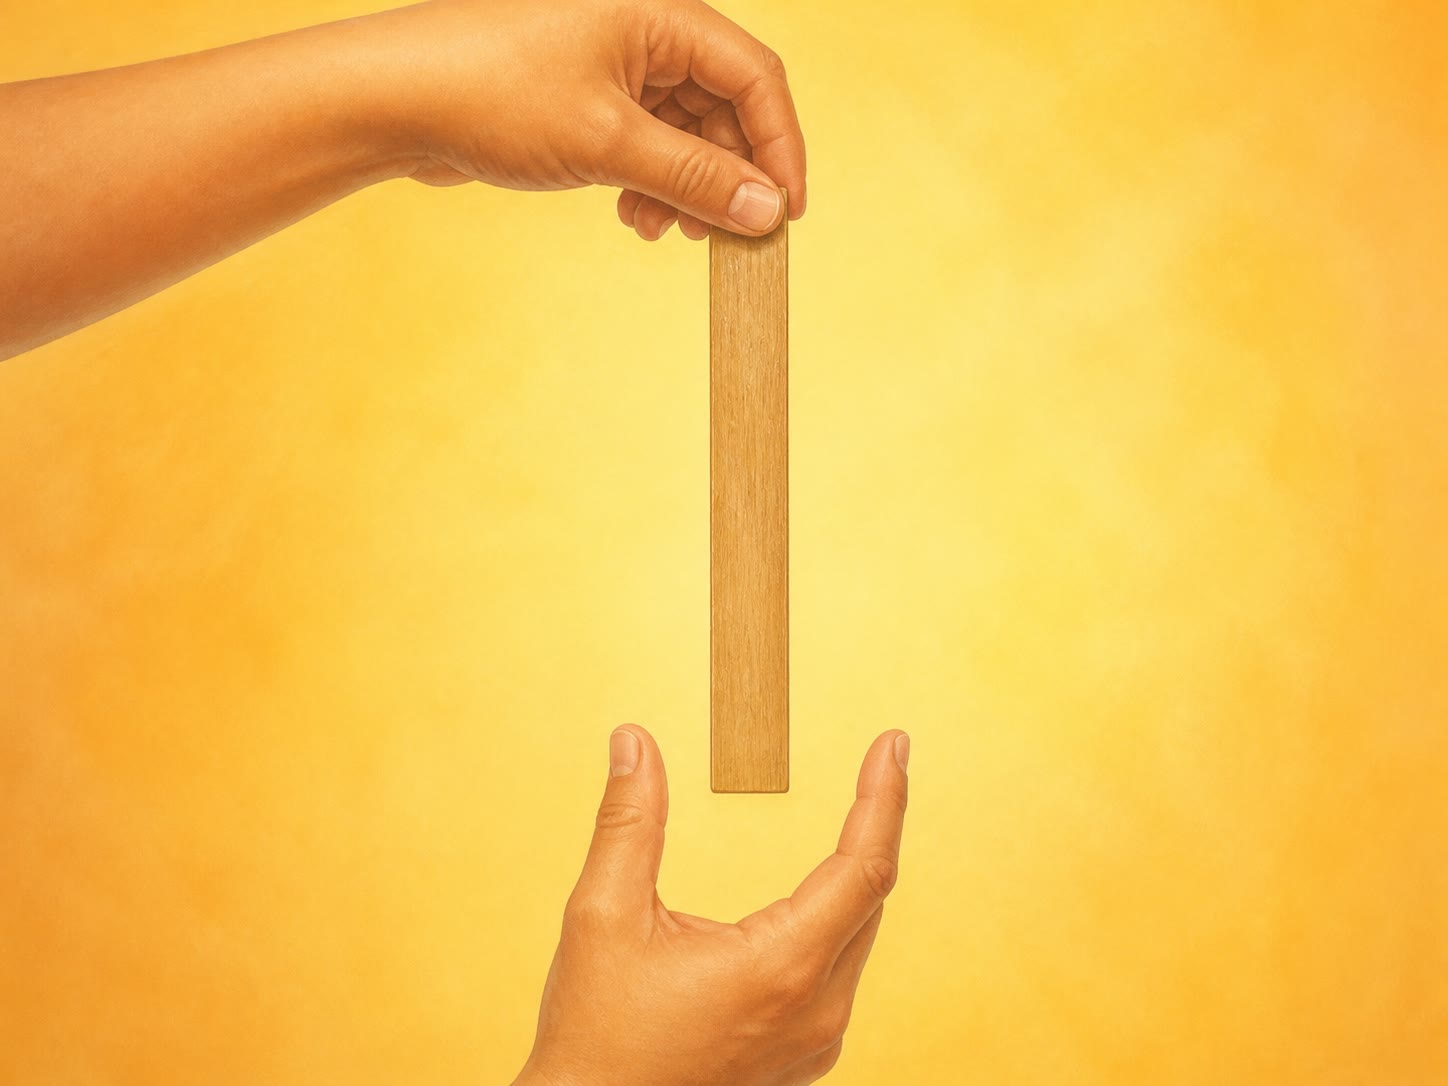
\includegraphics[width=0.5\linewidth]{images/book1/ai/g5-brain-ruler.jpg}

{\small 尺子测试，尺子落下的前一刻：上方的手松开时，
下方那只手的循环——看见、判断、
合上——开始它那五分之一秒。}
\end{omfigure}

\begin{example}[为什么副驾驶座上的人先倒吸凉气]\label{ex:g5:brain-in-command:driver}
五分之一秒似乎不算什么——直到速度把它放大
倍。高速公路车速下的汽车，约行驶\qty{7}{m}，在五分之一秒的
\omterm{def:g5:brain-in-command:reaction}{反应时间}内，驾驶员还没碰到刹车，
汽车已驶过一间教室的长度。\omterm{def:g5:brain-in-command:reaction}{反应
时间}正是车与车之间需要保持距离的原因，也是
驾驶员注意力是一个安全器官的缘由。
\end{example}

\begin{remark}[训练循环]\label{rem:g5:brain-in-command:training}
练习能缩短并磨快这个循环——改变的不是\omterm{def:g5:brain-in-command:system}{神经}的
传导速度，而是\omterm{def:g5:brain-in-command:system}{大脑}的调度方式。初学抛接球的人会把
球全部掉下；一个月后，同一个\omterm{def:g5:brain-in-command:system}{大脑}指挥同样的
双手抛接三个球，似乎毫不费力。学习
一项技能，就是\omterm{def:g5:brain-in-command:system}{大脑}铺设更好的通路——还有一样
也会随锻炼而增长的东西，像
\cref{met:g3:bones-and-muscles:care} 中的\omterm{def:g3:bones-and-muscles:muscle}{肌肉}那样。
\end{remark}

\section{保护指挥官}

\begin{proposition}[睡眠、食物与安全]\label{prop:g5:brain-in-command:protect}
\omterm{def:g5:brain-in-command:system}{大脑}是人体受保护最严密的器官——\omterm{def:g3:bones-and-muscles:skeleton}{颅骨}如头盔，
\omterm{def:g4:classifying-animals:vertebrate}{脊柱}如支柱；同时它也是需求最高的器官：尽管
只占体重的一小部分，却消耗了全身很大一部分的
\omterm{prop:g3:balanced-diet:jobs}{能量}与氧气
（见\cref{prop:g4:heart-and-blood:carries}），它还会在
\emph{\omterm{prop:g1:healthy-habits:needs}{睡眠}}期间整理与修复。
疲惫的\omterm{def:g5:brain-in-command:system}{大脑}指挥能力很差（见\cref{prop:g1:healthy-habits:needs}）：
反应变慢，注意力分散，
判断也易急躁。
\end{proposition}
\admitted

\begin{example}[头盔是为了保护这个循环]\label{ex:g5:brain-in-command:helmet}
骨头可以愈合（见\cref{rem:g3:bones-and-muscles:alive}）；\omterm{def:g5:brain-in-command:system}{大脑}
组织一旦严重受伤，大多不能恢复。这正是
自行车头盔背后的考量：\omterm{def:g3:bones-and-muscles:skeleton}{颅骨}加泡沫，
用在人体自身保护可能不足之处。投入很小的保险，
保护着统管其他一切的器官。
\end{example}

\section{练习}

\begin{exercise}[$\star$]\label{exo:g5:brain-in-command:1}
说出\omterm{def:g5:brain-in-command:system}{神经系统}的三个组成部分，以及各自的
作用。
\end{exercise}

\begin{exercise}[$\star$]\label{exo:g5:brain-in-command:2}
用三个步骤说明每个动作的循环。哪些部分
负责传递信息，哪些负责判断，哪些负责执行？
\end{exercise}

\begin{exercise}[$\star$]\label{exo:g5:brain-in-command:3}
\omterm{def:g5:brain-in-command:system}{大脑}和\omterm{def:g5:brain-in-command:system}{脊髓}各自位于何处受保护，
分别由哪些\omterm{def:g3:bones-and-muscles:skeleton}{骨骼}保护？
\end{exercise}

\begin{exercise}[$\star$]\label{exo:g5:brain-in-command:4}
什么是\omterm{def:g5:brain-in-command:reaction}{反应时间}？请给出一个简单任务中
\omterm{def:g5:brain-in-command:reaction}{反应时间}的大致数值。
\end{exercise}

\begin{exercise}[$\star$]\label{exo:g5:brain-in-command:5}
请按 \cref{ex:g5:brain-in-command:catch} 的方式慢慢回放：
你踩到尖锐的东西，脚猛地缩回。谁
负责传递信息，谁负责判断，谁负责执行？
\end{exercise}

\begin{exercise}[$\star$]\label{exo:g5:brain-in-command:6}
请列举\omterm{def:g5:brain-in-command:system}{大脑}在你无需思考时仍在运行的两项功能，
（见\cref{rem:g5:brain-in-command:more}）。
\end{exercise}

\begin{exercise}[$\star$]\label{exo:g5:brain-in-command:7}
为什么疲惫的\omterm{def:g5:brain-in-command:system}{大脑}指挥能力差？请说出
其中两项需求（见\cref{prop:g5:brain-in-command:protect}）。
\end{exercise}

\begin{exercise}[$\star$]\label{exo:g5:brain-in-command:8}
动手试一试：
\cref{met:g5:brain-in-command:ruler} 中的尺子测试，做五次，记录
你通常的接住距离——以及练习
是否使它有所改善。
\end{exercise}

\begin{exercise}[$\star\star$]\label{exo:g5:brain-in-command:9}
无论接球的人多熟练，为什么不存在
瞬间接住的情况？请用循环的三个步骤作答。
\end{exercise}

\begin{exercise}[$\star\star$]\label{exo:g5:brain-in-command:10}
请运用\cref{ex:g5:brain-in-command:driver}：为什么道路交通规则
要求车辆之间保持\emph{距离}，而不只是
仅仅要求刹车良好？注意力会改变循环中的
什么？
\end{exercise}

\begin{exercise}[$\star\star\star$]\label{exo:g5:brain-in-command:11}
\cref{rem:g5:brain-in-command:training} 中的杂耍者
她的\omterm{def:g5:brain-in-command:system}{神经}传导并没有变快，却仍然进步了。循环中的
哪一部分反而改善了？与训练\omterm{def:g3:bones-and-muscles:muscle}{肌肉}相比，
两种情况下各有什么在增长？
\end{exercise}
